\documentclass[tikz,border=2pt]{standalone}
\usepackage{amsmath,amssymb}
\usepackage{tikz}
\usetikzlibrary{arrows.meta}

\begin{document}
% In R^3 the span of one vector is a line through the origin, the span of two independent
% vectors is a plane through the origin.
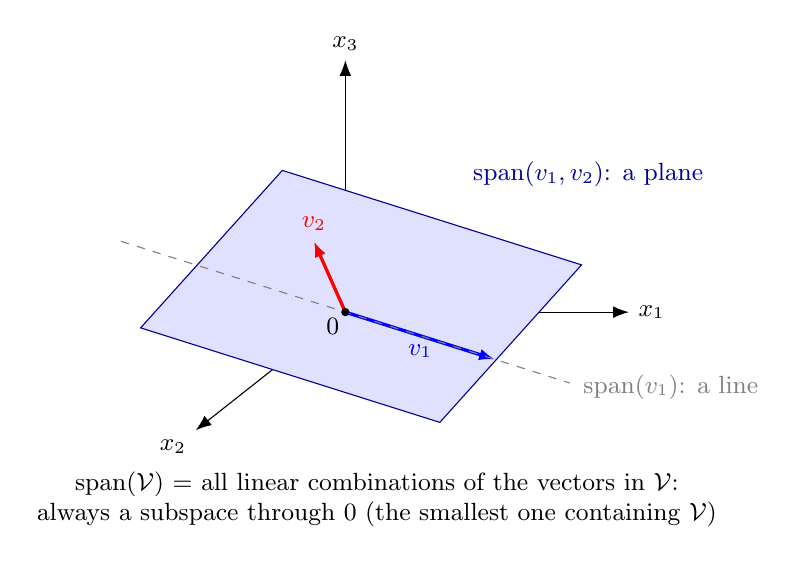
\begin{tikzpicture}[every node/.style={font=\small}, >={Latex[length=2mm]}]
	\draw[->] (0,0) -- (3.6,0) node[right] {$x_1$};
	\draw[->] (0,0) -- (0,3.2) node[above] {$x_3$};
	\draw[->] (0,0) -- (-1.9,-1.5) node[below left] {$x_2$};
	\fill[blue!12] (-2.6,-0.2) -- (1.2,-1.4) -- (3.0,0.6) -- (-0.8,1.8) -- cycle;
	\draw[blue!60!black] (-2.6,-0.2) -- (1.2,-1.4) -- (3.0,0.6) -- (-0.8,1.8) -- cycle;
	\draw[->, blue, very thick] (0,0) -- (1.9,-0.6) node[midway, below, inner sep=2.5pt] {$v_1$};
	\draw[->, red, very thick] (0,0) -- (-0.4,0.9) node[above] {$v_2$};
	\draw[gray, dashed] (-2.85,0.9) -- (2.85,-0.9);
	\node[blue!60!black, font=\small, anchor=west] at (1.5,1.75) {$\operatorname{span}(v_1,v_2)$: a plane};
	\node[gray, font=\small, anchor=west] at (2.9,-0.95) {$\operatorname{span}(v_1)$: a line};
	\fill (0,0) circle (1.5pt) node[below left, inner sep=2pt, font=\small] {$0$};
	\node[anchor=north, align=center] at (0.4,-1.9) {$\operatorname{span}(\mathcal{V})$ = all linear combinations of the vectors in $\mathcal{V}$:\\ always a subspace through $0$ (the smallest one containing $\mathcal{V}$)};
\end{tikzpicture}
\end{document}
